\documentclass[twoside]{book}

% Packages required by doxygen
\usepackage{fixltx2e}
\usepackage{calc}
\usepackage{doxygen}
\usepackage[export]{adjustbox} % also loads graphicx
\usepackage{graphicx}
\usepackage[utf8]{inputenc}
\usepackage{makeidx}
\usepackage{multicol}
\usepackage{multirow}
\PassOptionsToPackage{warn}{textcomp}
\usepackage{textcomp}
\usepackage[nointegrals]{wasysym}
\usepackage[table]{xcolor}

% Font selection
\usepackage[T1]{fontenc}
\usepackage[scaled=.90]{helvet}
\usepackage{courier}
\usepackage{amssymb}
\usepackage{sectsty}
\renewcommand{\familydefault}{\sfdefault}
\allsectionsfont{%
  \fontseries{bc}\selectfont%
  \color{darkgray}%
}
\renewcommand{\DoxyLabelFont}{%
  \fontseries{bc}\selectfont%
  \color{darkgray}%
}
\newcommand{\+}{\discretionary{\mbox{\scriptsize$\hookleftarrow$}}{}{}}

% Page & text layout
\usepackage{geometry}
\geometry{%
  a4paper,%
  top=2.5cm,%
  bottom=2.5cm,%
  left=2.5cm,%
  right=2.5cm%
}
\tolerance=750
\hfuzz=15pt
\hbadness=750
\setlength{\emergencystretch}{15pt}
\setlength{\parindent}{0cm}
\setlength{\parskip}{0.2cm}
\makeatletter
\renewcommand{\paragraph}{%
  \@startsection{paragraph}{4}{0ex}{-1.0ex}{1.0ex}{%
    \normalfont\normalsize\bfseries\SS@parafont%
  }%
}
\renewcommand{\subparagraph}{%
  \@startsection{subparagraph}{5}{0ex}{-1.0ex}{1.0ex}{%
    \normalfont\normalsize\bfseries\SS@subparafont%
  }%
}
\makeatother

% Headers & footers
\usepackage{fancyhdr}
\pagestyle{fancyplain}
\fancyhead[LE]{\fancyplain{}{\bfseries\thepage}}
\fancyhead[CE]{\fancyplain{}{}}
\fancyhead[RE]{\fancyplain{}{\bfseries\leftmark}}
\fancyhead[LO]{\fancyplain{}{\bfseries\rightmark}}
\fancyhead[CO]{\fancyplain{}{}}
\fancyhead[RO]{\fancyplain{}{\bfseries\thepage}}
\fancyfoot[LE]{\fancyplain{}{}}
\fancyfoot[CE]{\fancyplain{}{}}
\fancyfoot[RE]{\fancyplain{}{\bfseries\scriptsize Generated on Mon Jun 8 2015 08\+:29\+:55 for Collect-\/i\+O\+S by Doxygen }}
\fancyfoot[LO]{\fancyplain{}{\bfseries\scriptsize Generated on Mon Jun 8 2015 08\+:29\+:55 for Collect-\/i\+O\+S by Doxygen }}
\fancyfoot[CO]{\fancyplain{}{}}
\fancyfoot[RO]{\fancyplain{}{}}
\renewcommand{\footrulewidth}{0.4pt}
\renewcommand{\chaptermark}[1]{%
  \markboth{#1}{}%
}
\renewcommand{\sectionmark}[1]{%
  \markright{\thesection\ #1}%
}

% Indices & bibliography
\usepackage{natbib}
\usepackage[titles]{tocloft}
\setcounter{tocdepth}{3}
\setcounter{secnumdepth}{5}
\makeindex

% Hyperlinks (required, but should be loaded last)
\usepackage{ifpdf}
\ifpdf
  \usepackage[pdftex,pagebackref=true]{hyperref}
\else
  \usepackage[ps2pdf,pagebackref=true]{hyperref}
\fi
\hypersetup{%
  colorlinks=true,%
  linkcolor=blue,%
  citecolor=blue,%
  unicode%
}

% Custom commands
\newcommand{\clearemptydoublepage}{%
  \newpage{\pagestyle{empty}\cleardoublepage}%
}


%===== C O N T E N T S =====

\begin{document}

% Titlepage & ToC
\hypersetup{pageanchor=false,
             bookmarks=true,
             bookmarksnumbered=true,
             pdfencoding=unicode
            }
\pagenumbering{roman}
\begin{titlepage}
\vspace*{7cm}
\begin{center}%
{\Large Collect-\/i\+O\+S }\\
\vspace*{1cm}
{\large Generated by Doxygen 1.8.9.1}\\
\vspace*{0.5cm}
{\small Mon Jun 8 2015 08:29:55}\\
\end{center}
\end{titlepage}
\clearemptydoublepage
\tableofcontents
\clearemptydoublepage
\pagenumbering{arabic}
\hypersetup{pageanchor=true}

%--- Begin generated contents ---
\chapter{Hierarchical Index}
\section{Class Hierarchy}
This inheritance list is sorted roughly, but not completely, alphabetically\+:\begin{DoxyCompactList}
\item N\+S\+Object\begin{DoxyCompactList}
\item \contentsline{section}{T\+E\+A\+L\+Collect\+Configuration}{\pageref{interface_t_e_a_l_collect_configuration}}{}
\item \contentsline{section}{Tealium\+Collect}{\pageref{interface_tealium_collect}}{}
\end{DoxyCompactList}
\item $<$T\+E\+A\+L\+Collect\+Dispatch\+Manager\+Configuration$>$\begin{DoxyCompactList}
\item \contentsline{section}{Tealium\+Collect()}{\pageref{category_tealium_collect_07_08}}{}
\end{DoxyCompactList}
\item $<$T\+E\+A\+L\+Collect\+Dispatch\+Manager\+Delegate$>$\begin{DoxyCompactList}
\item \contentsline{section}{Tealium\+Collect()}{\pageref{category_tealium_collect_07_08}}{}
\end{DoxyCompactList}
\item $<$T\+E\+A\+L\+Settings\+Store\+Configuration$>$\begin{DoxyCompactList}
\item \contentsline{section}{Tealium\+Collect()}{\pageref{category_tealium_collect_07_08}}{}
\end{DoxyCompactList}
\end{DoxyCompactList}

\chapter{Class Index}
\section{Class List}
Here are the classes, structs, unions and interfaces with brief descriptions\+:\begin{DoxyCompactList}
\item\contentsline{section}{\hyperlink{interface_t_e_a_l_collect_configuration}{T\+E\+A\+L\+Collect\+Configuration} }{\pageref{interface_t_e_a_l_collect_configuration}}{}
\item\contentsline{section}{\hyperlink{interface_tealium_collect}{Tealium\+Collect} }{\pageref{interface_tealium_collect}}{}
\item\contentsline{section}{\hyperlink{category_tealium_collect_07_08}{Tealium\+Collect()} }{\pageref{category_tealium_collect_07_08}}{}
\end{DoxyCompactList}

\chapter{Class Documentation}
\hypertarget{interface_t_e_a_l_collect_configuration}{}\section{T\+E\+A\+L\+Collect\+Configuration Class Reference}
\label{interface_t_e_a_l_collect_configuration}\index{T\+E\+A\+L\+Collect\+Configuration@{T\+E\+A\+L\+Collect\+Configuration}}
Inheritance diagram for T\+E\+A\+L\+Collect\+Configuration\+:\begin{figure}[H]
\begin{center}
\leavevmode
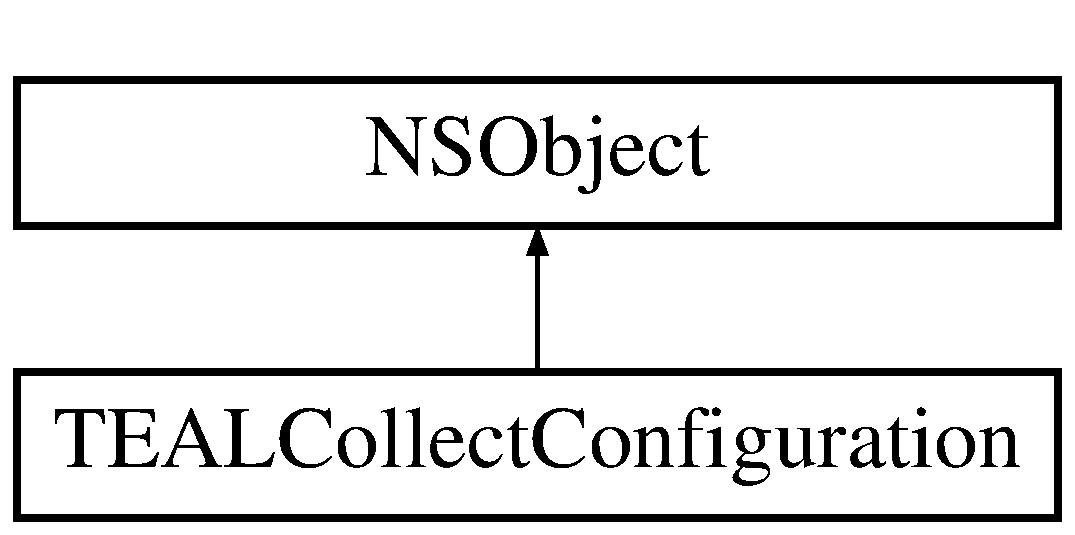
\includegraphics[height=2.000000cm]{interface_t_e_a_l_collect_configuration}
\end{center}
\end{figure}
\subsection*{Class Methods}
\begin{DoxyCompactItemize}
\item 
(instancetype) + \hyperlink{interface_t_e_a_l_collect_configuration_a6eec21b4797e86df33cd94b4d60f1bb5}{configuration\+With\+Account\+:profile\+:environment\+:}
\end{DoxyCompactItemize}
\subsection*{Properties}
\begin{DoxyCompactItemize}
\item 
\hypertarget{interface_t_e_a_l_collect_configuration_a40407bb324afffde3b7307f985614dba}{}N\+S\+String $\ast$ {\bfseries account\+Name}\label{interface_t_e_a_l_collect_configuration_a40407bb324afffde3b7307f985614dba}

\item 
\hypertarget{interface_t_e_a_l_collect_configuration_a69b64f0e1764f62acbb0fa558432eab9}{}N\+S\+String $\ast$ {\bfseries profile\+Name}\label{interface_t_e_a_l_collect_configuration_a69b64f0e1764f62acbb0fa558432eab9}

\item 
\hypertarget{interface_t_e_a_l_collect_configuration_aa40d0922a4edbfc0ae08456d1eae9a81}{}N\+S\+String $\ast$ {\bfseries environment\+Name}\label{interface_t_e_a_l_collect_configuration_aa40d0922a4edbfc0ae08456d1eae9a81}

\item 
\hypertarget{interface_t_e_a_l_collect_configuration_a9bca27197a89c7eb220c38046f55f0ec}{}B\+O\+O\+L {\bfseries use\+H\+T\+T\+P}\label{interface_t_e_a_l_collect_configuration_a9bca27197a89c7eb220c38046f55f0ec}

\item 
\hypertarget{interface_t_e_a_l_collect_configuration_a25a43a01198ac125fb2d3f49ad26bc7c}{}T\+E\+A\+L\+Profile\+Polling\+Frequency {\bfseries polling\+Frequency}\label{interface_t_e_a_l_collect_configuration_a25a43a01198ac125fb2d3f49ad26bc7c}

\item 
\hypertarget{interface_t_e_a_l_collect_configuration_a420d8d9420d62c3d26f2582491c03882}{}T\+E\+A\+L\+Collect\+Log\+Level {\bfseries log\+Level}\label{interface_t_e_a_l_collect_configuration_a420d8d9420d62c3d26f2582491c03882}

\item 
\hypertarget{interface_t_e_a_l_collect_configuration_a13e46e6e8c4c1e0756a5a91bf8a3d604}{}N\+S\+String $\ast$ {\bfseries audience\+Stream\+Profile}\label{interface_t_e_a_l_collect_configuration_a13e46e6e8c4c1e0756a5a91bf8a3d604}

\end{DoxyCompactItemize}


\subsection{Method Documentation}
\hypertarget{interface_t_e_a_l_collect_configuration_a6eec21b4797e86df33cd94b4d60f1bb5}{}\index{T\+E\+A\+L\+Collect\+Configuration@{T\+E\+A\+L\+Collect\+Configuration}!configuration\+With\+Account\+:profile\+:environment\+:@{configuration\+With\+Account\+:profile\+:environment\+:}}
\index{configuration\+With\+Account\+:profile\+:environment\+:@{configuration\+With\+Account\+:profile\+:environment\+:}!T\+E\+A\+L\+Collect\+Configuration@{T\+E\+A\+L\+Collect\+Configuration}}
\subsubsection[{configuration\+With\+Account\+:profile\+:environment\+:(\+N\+S\+String $\ast$account\+Name,[profile] N\+S\+String $\ast$profile\+Name,[environment] N\+S\+String $\ast$environment\+Name)}]{\setlength{\rightskip}{0pt plus 5cm}+ (instancetype) configuration\+With\+Account\+: 
\begin{DoxyParamCaption}
\item[{(N\+S\+String $\ast$)}]{account\+Name}
\item[{profile:(N\+S\+String $\ast$)}]{profile\+Name}
\item[{environment:(N\+S\+String $\ast$)}]{environment\+Name}
\end{DoxyParamCaption}
}\label{interface_t_e_a_l_collect_configuration_a6eec21b4797e86df33cd94b4d60f1bb5}
Creates a default configration instance for a given account / profile / environment combination. The Ti\+Q information is used to fetch the profile\textquotesingle{}s mobile publish settings used


\begin{DoxyParams}{Parameters}
{\em account\+Name} & String of Ti\+Q / Audience\+Stream account name \\
\hline
{\em profile\+Name} & String of Ti\+Q Profile Name \\
\hline
{\em environment\+Name} & String\\
\hline
\end{DoxyParams}
\begin{DoxyReturn}{Returns}
Valid configuration instance to pass to the enable\+With\+Configuration\+: method. 
\end{DoxyReturn}


The documentation for this class was generated from the following files\+:\begin{DoxyCompactItemize}
\item 
T\+E\+A\+L\+Collect\+Configuration.\+h\item 
T\+E\+A\+L\+Collect\+Configuration.\+m\end{DoxyCompactItemize}

\hypertarget{interface_tealium_collect}{}\section{Tealium\+Collect Class Reference}
\label{interface_tealium_collect}\index{Tealium\+Collect@{Tealium\+Collect}}
Inheritance diagram for Tealium\+Collect\+:\begin{figure}[H]
\begin{center}
\leavevmode
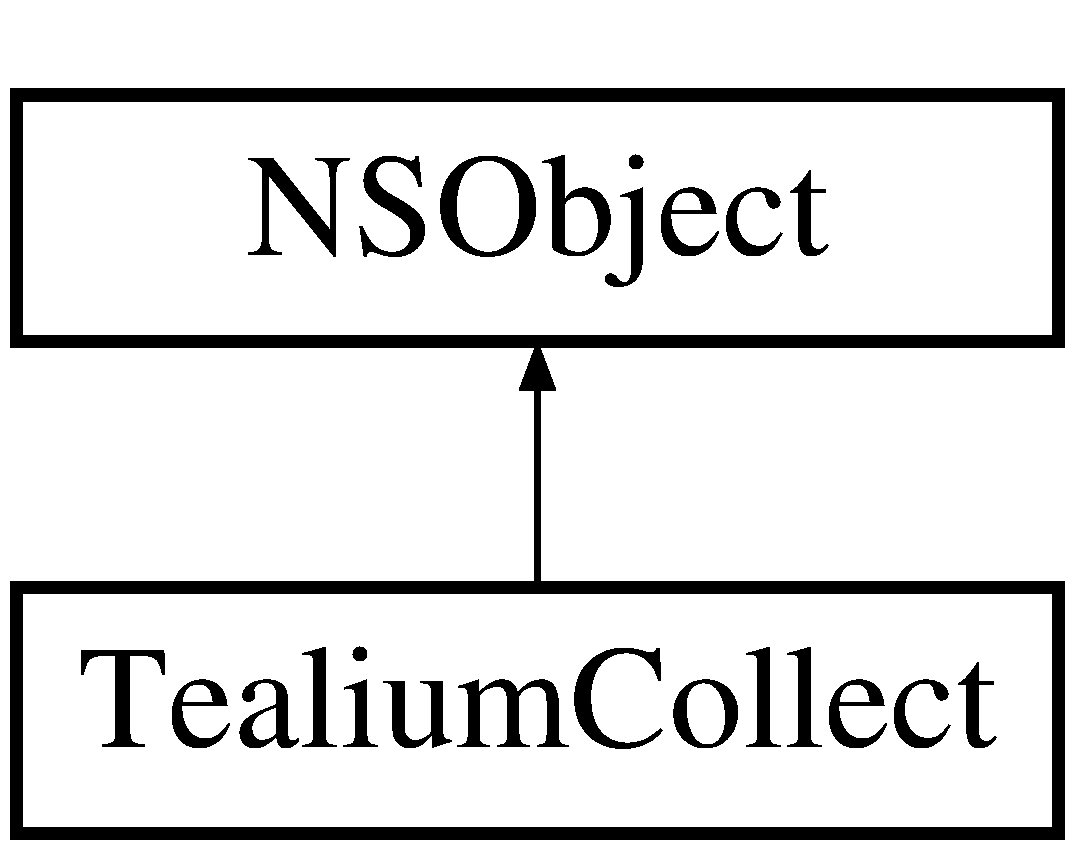
\includegraphics[height=2.000000cm]{interface_tealium_collect}
\end{center}
\end{figure}
\subsection*{Class Methods}
\begin{DoxyCompactItemize}
\item 
(void) + \hyperlink{interface_tealium_collect_abce36b787b0f702904bd3caaab7f1338}{enable\+With\+Configuration\+:}
\item 
(void) + \hyperlink{interface_tealium_collect_af6af3f00f06c027c116e7f401923ea8f}{enable\+With\+Configuration\+:completion\+:}
\item 
(void) + \hyperlink{interface_tealium_collect_ae44d61eeee08bde059a14fedd7ccb8fe}{disable}
\item 
(void) + \hyperlink{interface_tealium_collect_a22f691ac22d7337ed409400bb150e661}{send\+Event\+With\+Data\+:}
\item 
(void) + \hyperlink{interface_tealium_collect_a32cb460af6e28d696d773356503ff01e}{send\+View\+With\+Data\+:}
\item 
(void) + \hyperlink{interface_tealium_collect_a5e5d3f690eff622edcfaa89a39bf796d}{fetch\+Visitor\+Profile\+With\+Completion\+:}
\item 
(T\+E\+A\+L\+Visitor\+Profile $\ast$) + \hyperlink{interface_tealium_collect_ae65188d3776096b4e74d2fb0de43db64}{cached\+Visitor\+Profile\+Copy}
\item 
(N\+S\+String $\ast$) + \hyperlink{interface_tealium_collect_ada7cc24d226c7ad527eedfbd238dfec1}{visitor\+I\+D}
\item 
(void) + \hyperlink{interface_tealium_collect_a35aa38b8cdfa1cecb2083988334e9075}{join\+Trace\+With\+Token\+:}
\item 
(void) + \hyperlink{interface_tealium_collect_a05aabc4900b7d0095e96a30eb62b1ed0}{leave\+Trace}
\end{DoxyCompactItemize}


\subsection{Method Documentation}
\hypertarget{interface_tealium_collect_ae65188d3776096b4e74d2fb0de43db64}{}\index{Tealium\+Collect@{Tealium\+Collect}!cached\+Visitor\+Profile\+Copy@{cached\+Visitor\+Profile\+Copy}}
\index{cached\+Visitor\+Profile\+Copy@{cached\+Visitor\+Profile\+Copy}!Tealium\+Collect@{Tealium\+Collect}}
\subsubsection[{cached\+Visitor\+Profile\+Copy()}]{\setlength{\rightskip}{0pt plus 5cm}+ (T\+E\+A\+L\+Visitor\+Profile $\ast$) cached\+Visitor\+Profile\+Copy 
\begin{DoxyParamCaption}
{}
\end{DoxyParamCaption}
}\label{interface_tealium_collect_ae65188d3776096b4e74d2fb0de43db64}
Last retrieved profile instance. This is updated every time the profile is queried. Depending on the settings the library was enabled with, this could be after every send\+Event\+:custom\+Data\+: call or only on explicit request.

\begin{DoxyReturn}{Returns}
Returns valid T\+E\+A\+L\+Profile object. Its properties might be nil of nothing is loaded into them yet. 
\end{DoxyReturn}
\hypertarget{interface_tealium_collect_ae44d61eeee08bde059a14fedd7ccb8fe}{}\index{Tealium\+Collect@{Tealium\+Collect}!disable@{disable}}
\index{disable@{disable}!Tealium\+Collect@{Tealium\+Collect}}
\subsubsection[{disable()}]{\setlength{\rightskip}{0pt plus 5cm}+ (void) disable 
\begin{DoxyParamCaption}
{}
\end{DoxyParamCaption}
}\label{interface_tealium_collect_ae44d61eeee08bde059a14fedd7ccb8fe}
Disabled the library from operating. Sets the libraries internal state to disabled, all subsequent method calls with be ignored. \hypertarget{interface_tealium_collect_abce36b787b0f702904bd3caaab7f1338}{}\index{Tealium\+Collect@{Tealium\+Collect}!enable\+With\+Configuration\+:@{enable\+With\+Configuration\+:}}
\index{enable\+With\+Configuration\+:@{enable\+With\+Configuration\+:}!Tealium\+Collect@{Tealium\+Collect}}
\subsubsection[{enable\+With\+Configuration\+:(\+T\+E\+A\+L\+Collect\+Configuration $\ast$configuration)}]{\setlength{\rightskip}{0pt plus 5cm}+ (void) enable\+With\+Configuration\+: 
\begin{DoxyParamCaption}
\item[{({\bf T\+E\+A\+L\+Collect\+Configuration} $\ast$)}]{configuration}
\end{DoxyParamCaption}
}\label{interface_tealium_collect_abce36b787b0f702904bd3caaab7f1338}
Starts the Audience\+Stream Library with the given configuration object.


\begin{DoxyParams}{Parameters}
{\em configuration} & T\+E\+A\+L\+Audience\+Stream\+Configuration instance with valid Account/\+Profile/\+Enviroment properties. \\
\hline
\end{DoxyParams}
\hypertarget{interface_tealium_collect_af6af3f00f06c027c116e7f401923ea8f}{}\index{Tealium\+Collect@{Tealium\+Collect}!enable\+With\+Configuration\+:completion\+:@{enable\+With\+Configuration\+:completion\+:}}
\index{enable\+With\+Configuration\+:completion\+:@{enable\+With\+Configuration\+:completion\+:}!Tealium\+Collect@{Tealium\+Collect}}
\subsubsection[{enable\+With\+Configuration\+:completion\+:(\+T\+E\+A\+L\+Collect\+Configuration $\ast$configuration,[completion] T\+E\+A\+L\+Boolean\+Completion\+Block completion)}]{\setlength{\rightskip}{0pt plus 5cm}+ (void) {\bf enable\+With\+Configuration\+:} 
\begin{DoxyParamCaption}
\item[{({\bf T\+E\+A\+L\+Collect\+Configuration} $\ast$)}]{configuration}
\item[{completion:(T\+E\+A\+L\+Boolean\+Completion\+Block)}]{completion}
\end{DoxyParamCaption}
}\label{interface_tealium_collect_af6af3f00f06c027c116e7f401923ea8f}
Starts the Audience\+Stream Library with the given configuration object.


\begin{DoxyParams}{Parameters}
{\em configuration} & T\+E\+A\+L\+Audience\+Stream\+Configuration instance with valid Account/\+Profile/\+Enviroment properties. \\
\hline
{\em completion} & T\+E\+A\+L\+Boolean\+Completion\+Block which is called after settings have loaded and visitor\+I\+D has been created or restored. \\
\hline
\end{DoxyParams}
\hypertarget{interface_tealium_collect_a5e5d3f690eff622edcfaa89a39bf796d}{}\index{Tealium\+Collect@{Tealium\+Collect}!fetch\+Visitor\+Profile\+With\+Completion\+:@{fetch\+Visitor\+Profile\+With\+Completion\+:}}
\index{fetch\+Visitor\+Profile\+With\+Completion\+:@{fetch\+Visitor\+Profile\+With\+Completion\+:}!Tealium\+Collect@{Tealium\+Collect}}
\subsubsection[{fetch\+Visitor\+Profile\+With\+Completion\+:(void($^\wedge$completion)(\+T\+E\+A\+L\+Visitor\+Profile $\ast$profile, N\+S\+Error $\ast$error))}]{\setlength{\rightskip}{0pt plus 5cm}+ (void) fetch\+Visitor\+Profile\+With\+Completion\+: 
\begin{DoxyParamCaption}
\item[{(void($^\wedge$)(T\+E\+A\+L\+Visitor\+Profile $\ast$profile, N\+S\+Error $\ast$error))}]{completion}
\end{DoxyParamCaption}
}\label{interface_tealium_collect_a5e5d3f690eff622edcfaa89a39bf796d}
Retrieves the current visitor profile from Audience\+Stream.


\begin{DoxyParams}{Parameters}
{\em completion} & Completion block with retrieved T\+E\+A\+L\+Profile instance and an error should any problems occur. \\
\hline
\end{DoxyParams}
\hypertarget{interface_tealium_collect_a35aa38b8cdfa1cecb2083988334e9075}{}\index{Tealium\+Collect@{Tealium\+Collect}!join\+Trace\+With\+Token\+:@{join\+Trace\+With\+Token\+:}}
\index{join\+Trace\+With\+Token\+:@{join\+Trace\+With\+Token\+:}!Tealium\+Collect@{Tealium\+Collect}}
\subsubsection[{join\+Trace\+With\+Token\+:(\+N\+S\+String $\ast$token)}]{\setlength{\rightskip}{0pt plus 5cm}+ (void) join\+Trace\+With\+Token\+: 
\begin{DoxyParamCaption}
\item[{(N\+S\+String $\ast$)}]{token}
\end{DoxyParamCaption}
}\label{interface_tealium_collect_a35aa38b8cdfa1cecb2083988334e9075}
Joins a trace initiated from the Audience\+Stream web app with a valid string token provide from the Trace\+U\+I


\begin{DoxyParams}{Parameters}
{\em token} & String value should match the code provided via the Audience\+Stream web U\+I. \\
\hline
\end{DoxyParams}
\hypertarget{interface_tealium_collect_a05aabc4900b7d0095e96a30eb62b1ed0}{}\index{Tealium\+Collect@{Tealium\+Collect}!leave\+Trace@{leave\+Trace}}
\index{leave\+Trace@{leave\+Trace}!Tealium\+Collect@{Tealium\+Collect}}
\subsubsection[{leave\+Trace()}]{\setlength{\rightskip}{0pt plus 5cm}+ (void) leave\+Trace 
\begin{DoxyParamCaption}
{}
\end{DoxyParamCaption}
}\label{interface_tealium_collect_a05aabc4900b7d0095e96a30eb62b1ed0}
Stops sending trace data for the provided token in the join\+Trace\+With\+Token\+: method. \hypertarget{interface_tealium_collect_a22f691ac22d7337ed409400bb150e661}{}\index{Tealium\+Collect@{Tealium\+Collect}!send\+Event\+With\+Data\+:@{send\+Event\+With\+Data\+:}}
\index{send\+Event\+With\+Data\+:@{send\+Event\+With\+Data\+:}!Tealium\+Collect@{Tealium\+Collect}}
\subsubsection[{send\+Event\+With\+Data\+:(\+N\+S\+Dictionary $\ast$custom\+Data)}]{\setlength{\rightskip}{0pt plus 5cm}+ (void) send\+Event\+With\+Data\+: 
\begin{DoxyParamCaption}
\item[{(N\+S\+Dictionary $\ast$)}]{custom\+Data}
\end{DoxyParamCaption}
}\label{interface_tealium_collect_a22f691ac22d7337ed409400bb150e661}
Sends an event to Audience\+Stream. Event are packaged with any custom key/value data sources passed in along with the default datasources provided by the library.


\begin{DoxyParams}{Parameters}
{\em custom\+Data} & Dictionary of custom datasources (key/value pairs) to be included in the event dispatch. \\
\hline
\end{DoxyParams}
\hypertarget{interface_tealium_collect_a32cb460af6e28d696d773356503ff01e}{}\index{Tealium\+Collect@{Tealium\+Collect}!send\+View\+With\+Data\+:@{send\+View\+With\+Data\+:}}
\index{send\+View\+With\+Data\+:@{send\+View\+With\+Data\+:}!Tealium\+Collect@{Tealium\+Collect}}
\subsubsection[{send\+View\+With\+Data\+:(\+N\+S\+Dictionary $\ast$custom\+Data)}]{\setlength{\rightskip}{0pt plus 5cm}+ (void) send\+View\+With\+Data\+: 
\begin{DoxyParamCaption}
\item[{(N\+S\+Dictionary $\ast$)}]{custom\+Data}
\end{DoxyParamCaption}
}\label{interface_tealium_collect_a32cb460af6e28d696d773356503ff01e}
Sends a view to Audience\+Stream. Views are packaged with any custom key/value data sources passed in along with the default datasources provided by the library.


\begin{DoxyParams}{Parameters}
{\em custom\+Data} & Dictionary of custom datasources (key/value pairs) to be included in the event dispatch. \\
\hline
\end{DoxyParams}
\hypertarget{interface_tealium_collect_ada7cc24d226c7ad527eedfbd238dfec1}{}\index{Tealium\+Collect@{Tealium\+Collect}!visitor\+I\+D@{visitor\+I\+D}}
\index{visitor\+I\+D@{visitor\+I\+D}!Tealium\+Collect@{Tealium\+Collect}}
\subsubsection[{visitor\+I\+D()}]{\setlength{\rightskip}{0pt plus 5cm}+ (N\+S\+String $\ast$) visitor\+I\+D 
\begin{DoxyParamCaption}
{}
\end{DoxyParamCaption}
}\label{interface_tealium_collect_ada7cc24d226c7ad527eedfbd238dfec1}
Unique visitor I\+D per Account / Device combination.

\begin{DoxyReturn}{Returns}
String value of the visitor\+I\+D for the Account the library was enabled with. 
\end{DoxyReturn}


The documentation for this class was generated from the following files\+:\begin{DoxyCompactItemize}
\item 
Tealium\+Collect.\+h\item 
Tealium\+Collect.\+m\end{DoxyCompactItemize}

\hypertarget{category_tealium_collect_07_08}{}\section{Tealium\+Collect() Category Reference}
\label{category_tealium_collect_07_08}\index{Tealium\+Collect()@{Tealium\+Collect()}}
Inheritance diagram for Tealium\+Collect()\+:\begin{figure}[H]
\begin{center}
\leavevmode
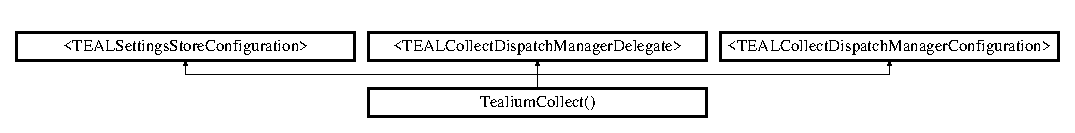
\includegraphics[height=1.333333cm]{category_tealium_collect_07_08}
\end{center}
\end{figure}
\subsection*{Properties}
\begin{DoxyCompactItemize}
\item 
\hypertarget{category_tealium_collect_07_08_aec8a4b574547743e8718591b76418dfa}{}T\+E\+A\+L\+Settings\+Store $\ast$ {\bfseries settings\+Store}\label{category_tealium_collect_07_08_aec8a4b574547743e8718591b76418dfa}

\item 
\hypertarget{category_tealium_collect_07_08_a5fe505345005d2dcd619b41f86fb7e0f}{}T\+E\+A\+L\+Collect\+Dispatch\+Manager $\ast$ {\bfseries dispatch\+Manager}\label{category_tealium_collect_07_08_a5fe505345005d2dcd619b41f86fb7e0f}

\item 
\hypertarget{category_tealium_collect_07_08_a405f95e8e980383aa16d498ba5fe3541}{}T\+E\+A\+L\+Profile\+Store $\ast$ {\bfseries profile\+Store}\label{category_tealium_collect_07_08_a405f95e8e980383aa16d498ba5fe3541}

\item 
\hypertarget{category_tealium_collect_07_08_a7ec13629c5a3bc81c0e8ac34b14a2a7c}{}T\+E\+A\+L\+Datasource\+Store $\ast$ {\bfseries datasource\+Store}\label{category_tealium_collect_07_08_a7ec13629c5a3bc81c0e8ac34b14a2a7c}

\item 
\hypertarget{category_tealium_collect_07_08_a5f016b0c3f0c571354b8f1e7f7b70e6a}{}T\+E\+A\+L\+Operation\+Manager $\ast$ {\bfseries operation\+Manager}\label{category_tealium_collect_07_08_a5f016b0c3f0c571354b8f1e7f7b70e6a}

\item 
\hypertarget{category_tealium_collect_07_08_abf9b6a5a2b94a3b22395afe9bd3c5c5d}{}T\+E\+A\+L\+U\+R\+L\+Session\+Manager $\ast$ {\bfseries url\+Session\+Manager}\label{category_tealium_collect_07_08_abf9b6a5a2b94a3b22395afe9bd3c5c5d}

\item 
\hypertarget{category_tealium_collect_07_08_adba0d45acf9528df431a4012a963050c}{}N\+S\+String $\ast$ {\bfseries visitor\+I\+D}\label{category_tealium_collect_07_08_adba0d45acf9528df431a4012a963050c}

\item 
\hypertarget{category_tealium_collect_07_08_a8291122081db8a48ed3f3bc6d9def85e}{}T\+E\+A\+L\+Visitor\+Profile $\ast$ {\bfseries cached\+Profile}\label{category_tealium_collect_07_08_a8291122081db8a48ed3f3bc6d9def85e}

\item 
\hypertarget{category_tealium_collect_07_08_ac709770f5bb33c8b3957e155bbbd86c6}{}B\+O\+O\+L {\bfseries enabled}\label{category_tealium_collect_07_08_ac709770f5bb33c8b3957e155bbbd86c6}

\end{DoxyCompactItemize}


The documentation for this category was generated from the following file\+:\begin{DoxyCompactItemize}
\item 
Tealium\+Collect.\+m\end{DoxyCompactItemize}

%--- End generated contents ---

% Index
\backmatter
\newpage
\phantomsection
\clearemptydoublepage
\addcontentsline{toc}{chapter}{Index}
\printindex

\end{document}
